\section{Public Evidence: Six Arenas and Six Programs}
\label{sec:results}\label{sec:frontierevidence}

\begin{designbox}
Report every public result as a scoped claim under its exact protocol, with its
evidence status attached and human or paper-reported references first where available.
Units are never cross-normalized, a snapshot is never shown as a reproduced artifact,
and a paper count is never shown as accepted papers.
\end{designbox}

\subsection{What the evidence is for}

This section is the proof-point ledger for the qualified thesis of Act~III: two public
records --- six benchmark arenas~\cite{argus_results} and a 41-paper research
portfolio~\cite{argus_research} --- offered as evidence of \emph{breadth} across task
classes and \emph{depth} within a few of them, not of universal capability. Nothing
here is a scalar ``frontier score'' or a guarantee of correctness outside the stated
protocols.

\subsection{Six benchmark arenas}
\label{sec:arenas}

Argus publishes a live public record~\cite{argus_results}. Figure~\ref{fig:results}
presents its six current arena results as small multiples --- one panel per arena,
each with its own unit --- because the arenas measure different quantities (kernel
rank, bits-per-byte, wall-clock seconds, solve rate, a gap score) and any shared axis
would mislead. Table~\ref{tab:results} gives the exact protocol, result, published
comparison, and evidence status for each row.

\begin{figure}[H]
\centering

\includegraphics[width=0.62\textwidth]{figures/public_results.pdf}
\caption{Public results across six arenas, drawn deterministically from
\code{technical\_report/evidence/website\_results.json}. Panels are not
cross-normalized; each carries its own unit and evidence status. Direction is
shown where defined; Arbor retains the site's reported metric without inferring
its direction. Argus bars are indigo; human/system baselines are lighter.}
\label{fig:results}
\end{figure}

\begin{table}[H]
\centering
\small
\begin{tabularx}{\linewidth}{@{}p{2.5cm} p{2.7cm} p{2.15cm} X p{1.55cm}@{}}
\toprule
\textbf{Arena} & \textbf{Protocol} & \textbf{Argus result} & \textbf{Published comparison} & \textbf{Status} \\
\midrule
NVIDIA SOL-ExecBench & B200; 101 kernels & Global \#6; 2$\times$\#1; 7 top-3 & Global rank vs.\ all entrants (headline) & snapshot \\
nanochat (B200) & 5\,min; 1$\times$B200; 426 attempts & 0.9636 BPB & Human SOTA 0.9646 & \textbf{digest} \\
nanochat (H100) & 5\,min; 1$\times$H100; 37 mechanisms & 0.9855 BPB & Human SOTA 0.9879 & snapshot \\
nanoGPT speedrun & 8$\times$H100; $N{=}10$ & 79.77\,s & Same-device human \#83: 80.18\,s & \textbf{digest} \\
AARRI-Bench & 82 research-intern tasks & 63/82 (76.8\%) & Paper-reported best 68.3\% & snapshot \\
Arbor (RUC NLPIR) & Math-reasoning data & 28.0 gap & Arbor 20.83; Claude Code 8.33; Codex 6.25 & snapshot \\
\bottomrule
\end{tabularx}
\caption{The six public results~\cite{argus_results}, verbatim from the evidence
bundle. Human and paper-reported references are primary where available; the
SOL-ExecBench headline is its global rank. SOL-ExecBench and Arbor also preserve
the site's published system/agent comparisons. ``digest'' = committed artifact
metadata; ``snapshot'' = public website snapshot.}
\label{tab:results}
\end{table}

Each number means exactly what its protocol row says and nothing more: the
\textbf{SOL-ExecBench}~\cite{ouyang2025kernelbench} headline is a \emph{global rank}
against all entrants, with the two head-to-head wins over
Recursive~\cite{recursive2026firststeps} the site's note, not the framing; lower
bits-per-byte and fewer seconds are better on
\textbf{nanochat}~\cite{karpathy_nanochat} and the \textbf{nanoGPT
speedrun}~\cite{karpathy_nanogpt}; and for \textbf{Arbor} the snapshot leaves the
``gap'' metric's direction undefined, so the values are quoted without interpreting
the ordering.

\subsection{Reading evidence status}

Two of the six rows carry artifact-digest corroboration, stated rather than smoothed
over. The \textbf{nanoGPT} 79.77\,s row references an $N{=}10$ verifier-certified
artifact in the external \code{nanogpt-speedrun-h100} project --- \code{valid=true,
n=10}, validation loss $3.2776$, one-sided $p(\text{mean}<3.28)=0.0040$, train time
$79.77\pm0.06$\,s, \code{seal=ok}. The \textbf{nanochat B200} 0.9636 row records
frozen-scorer, single-seed \code{MEAN\_VAL\_BPB}$=0.963634$ with a frozen-scorer exit
code of 0 and a genuine SM100 flash-attention kernel, in the
\code{nanochat-mission-b200} project. This repository commits the logical artifact
IDs, verifier excerpts, and SHA-256 digests --- not the external artifact bytes. The
other four rows (SOL-ExecBench, nanochat H100, AARRI-Bench, Arbor) are
\code{website\_snapshot} linked to
\code{technical\_report/evidence/website\_results.json}; no corroboration file was
fabricated where artifact-digest metadata was unavailable.

\subsection{Six research programs}
\label{sec:portfolio}

Beyond the arenas, Argus runs an optional idea-to-submission research pipeline (the
\code{research} vertical) whose public output is a collection of \textbf{41
papers}~\cite{argus_research} --- 35 manuscripts and 6 drafts, with duplicate versions
removed --- across six research programs (Figure~\ref{fig:portfolio},
Table~\ref{tab:portfolio}).

\begin{figure}[H]
\centering
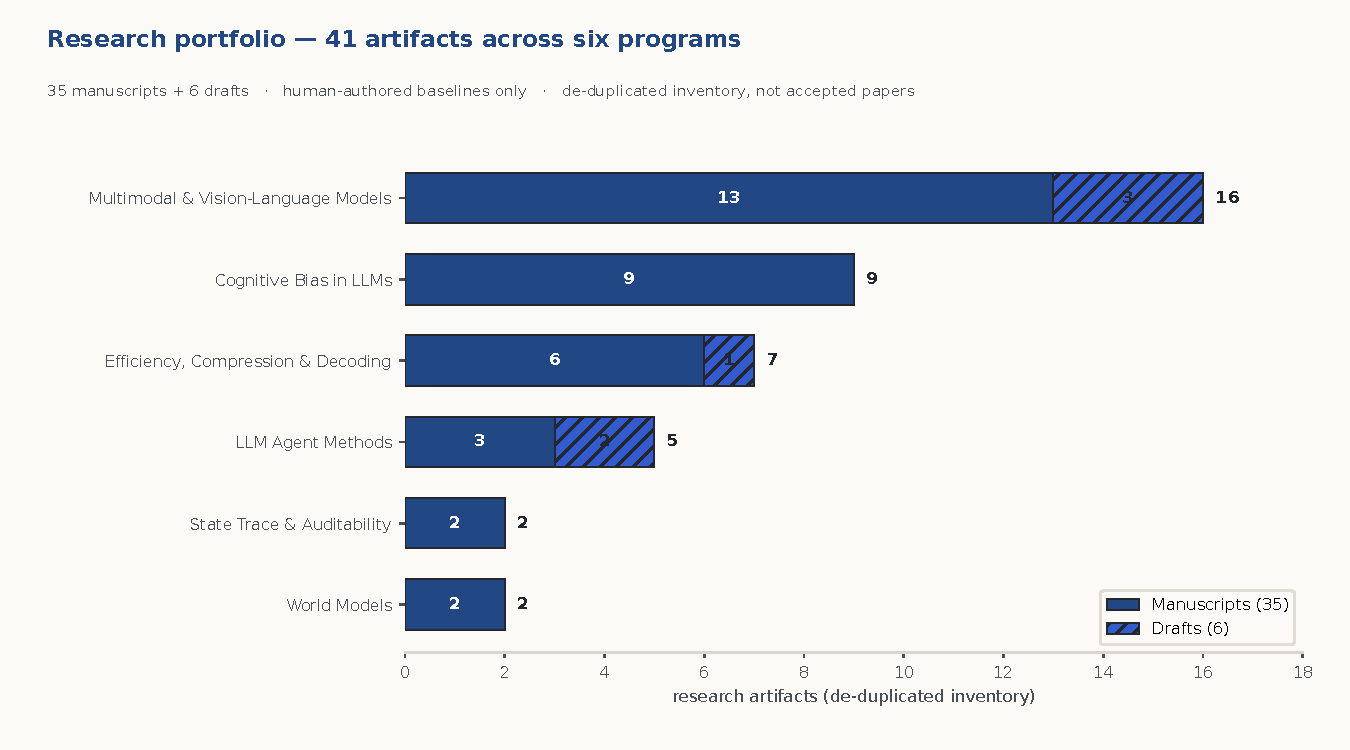
\includegraphics[width=0.50\textwidth]{figures/paper_portfolio.pdf}
\caption{The 41-paper portfolio by program and status, drawn deterministically from
\code{technical\_report/evidence/paper\_inventory.json}. Manuscripts are indigo,
drafts lighter. The count is a de-duplicated inventory compared only to
human-authored literature/baselines --- not a count of accepted papers.}
\label{fig:portfolio}
\end{figure}

\begin{table}[H]
\centering
\small
\begin{tabularx}{\linewidth}{@{}X r r r@{}}
\toprule
\textbf{Program} & \textbf{Manuscripts} & \textbf{Drafts} & \textbf{Total} \\
\midrule
Multimodal \& Vision-Language Models & 13 & 3 & 16 \\
Cognitive Bias in LLMs               &  9 & 0 &  9 \\
Efficiency, Compression \& Decoding  &  6 & 1 &  7 \\
LLM Agent Methods                    &  3 & 2 &  5 \\
World Models                         &  2 & 0 &  2 \\
State Trace \& Auditability          &  2 & 0 &  2 \\
\midrule
\textbf{Total}                       & \textbf{35} & \textbf{6} & \textbf{41} \\
\bottomrule
\end{tabularx}
\caption{Research portfolio by program and status~\cite{argus_research}. The
machine-readable inventory is
\code{technical\_report/evidence/paper\_inventory.json}.}
\label{tab:portfolio}
\end{table}

The portfolio concentrates in a few areas --- \textbf{Multimodal \& Vision-Language
Models} is the largest program --- and each paper is positioned against human-authored
literature and baselines, with the human comparison, where the site provides one,
preserved in the inventory (Table~\ref{tab:portfolio}).

\subsection{What 41 means}

Three qualifications keep the number honest. First, 41 is a \emph{de-duplicated
inventory} of research runs that produced a manuscript or draft, with duplicate
versions removed; it is not a count of accepted papers, and this report makes no
acceptance claim. Second, the 35 manuscripts and 6 drafts are reported as-is: a draft
is an in-progress artifact. Third, the collection is compared \emph{only} to
human-authored literature and baselines --- paper count and quality are never compared
to any other agent or model.

\subsection{Connection to the frontier thesis}

Read against the qualified frontier of Section~\ref{sec:frontier}: the arena results
are mostly \emph{depth within a domain} --- pushing one well-defined problem close to
or past a human or paper-reported reference on stated hardware --- while the portfolio
is mostly \emph{breadth across task classes}. The two are never combined into a single
scalar, so this report does not claim a universal capability index, a monotone
improvement curve, or that breadth and depth compose into general superiority. Each
cell is a scoped claim under its own protocol and evidence tier; converting the four
snapshot rows into artifact-digest records tied to a named commit is an explicit
roadmap item (Section~\ref{sec:roadmap}), and no row claims external peer-review
acceptance.
